Le diagramme suivant représente les élément logiciels les plus importants de notre architecture. Ces différents composants sont décrits en détail dans les sections suivantes.
\begin{figure}[H]
    \begin{center}
        \frame{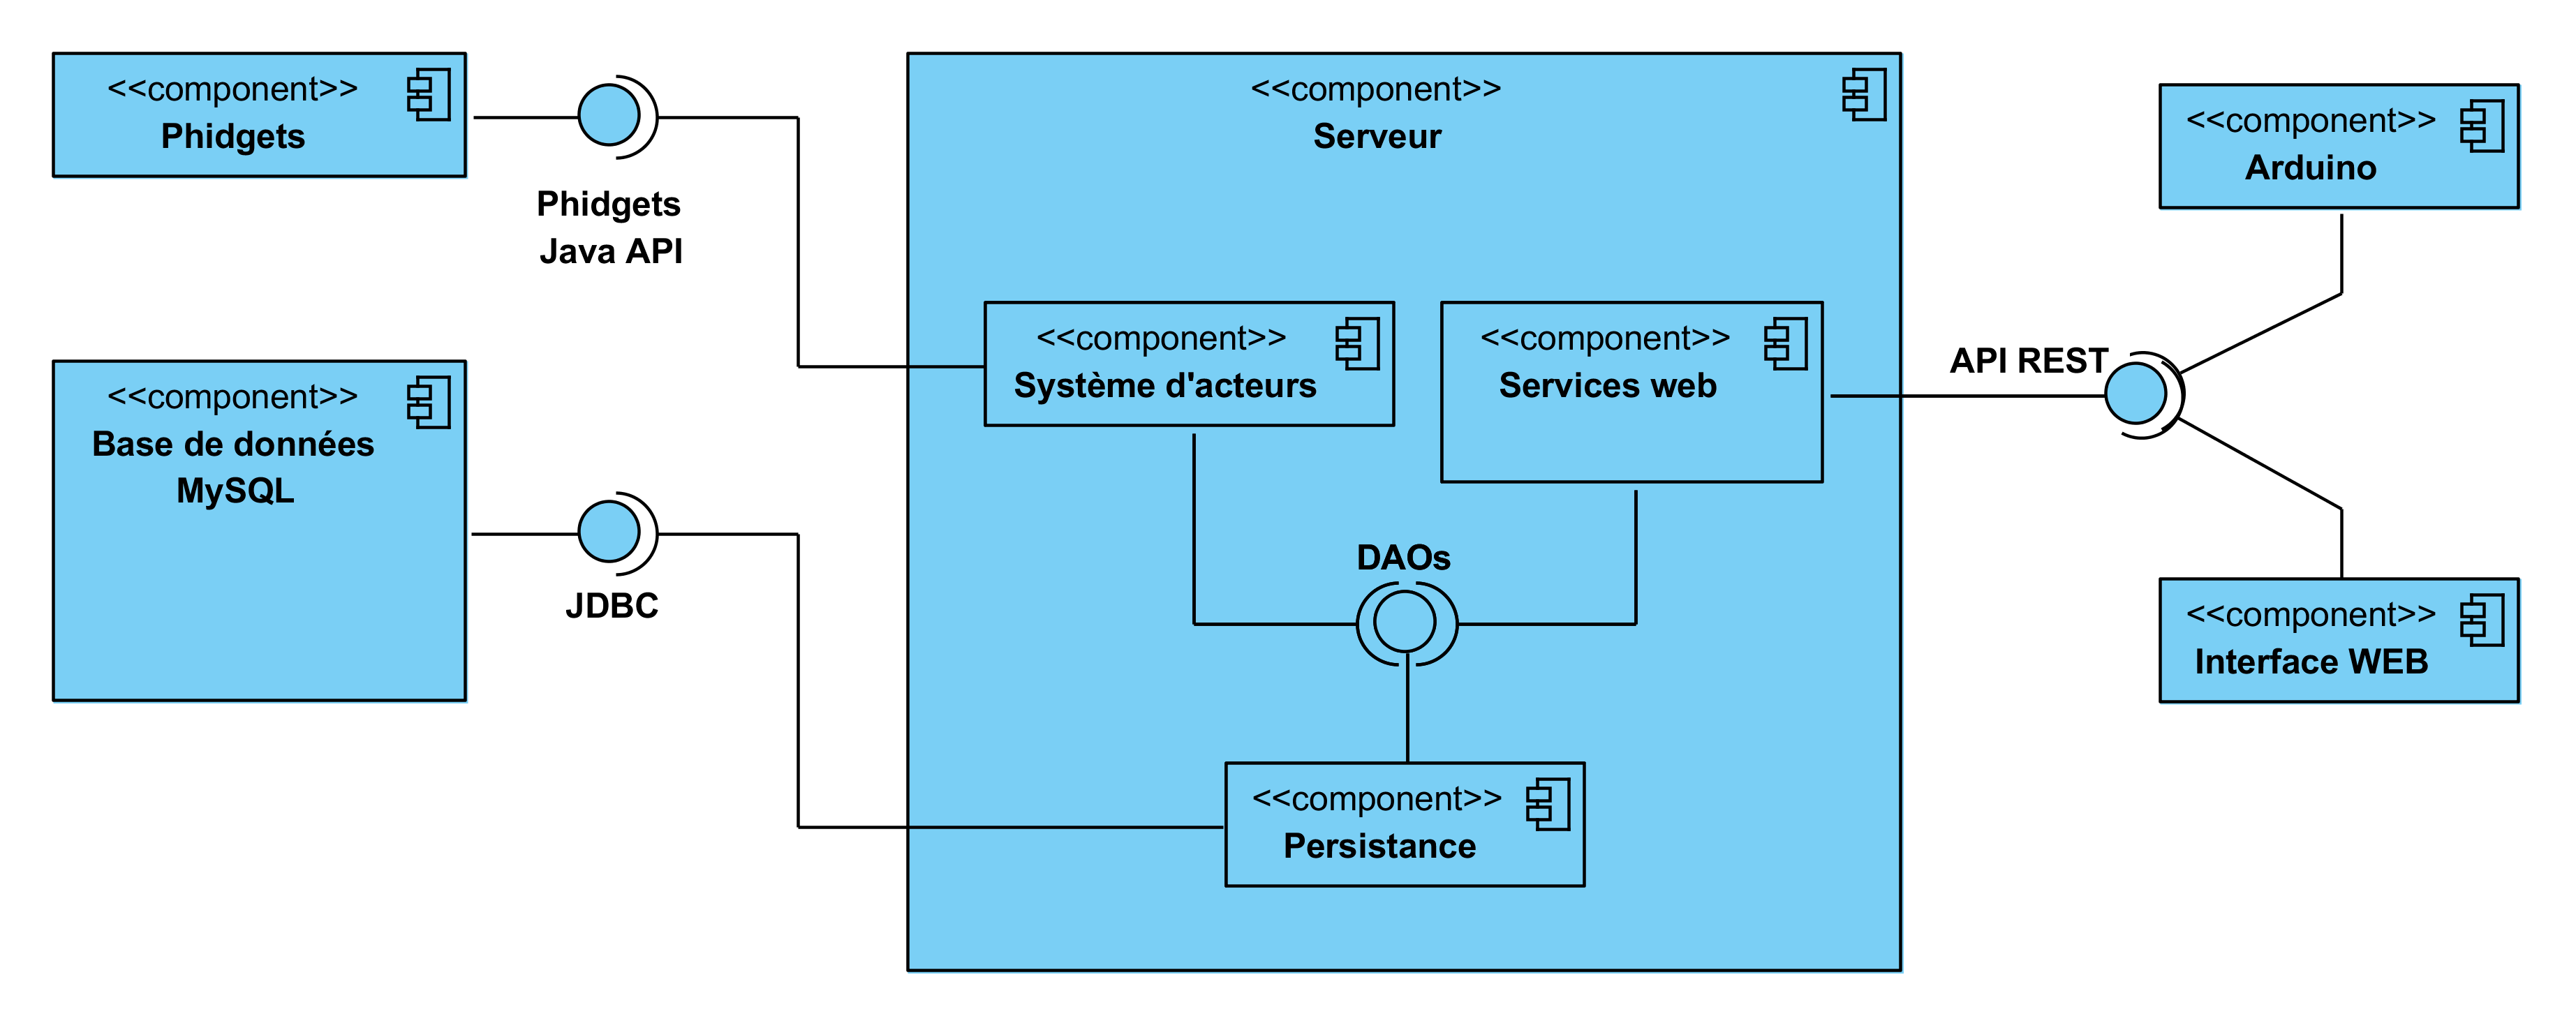
\includegraphics[width=\linewidth, height=\textheight,keepaspectratio]{img/diagramme-composants-archi-logi}}

        \caption{Diagramme de composants de l'architecture logicielle}
    \end{center}
\end{figure}
\subsection{Serveur}
Notre architecture logicielle côté serveur est basée sur une pile applicative reposant entièrement sur le langage Scala. Nous nous attarderons ici à décrire les 3 composants regroupés dans le serveur.\\

Néanmoins, quelques remarques préliminaires sont nécessaires :
\begin{itemize}
\item Pour faciliter le développement et surtout la gestion des dépendances, nous avons utilisé Maven. Lors de la phase de développement, le conteneur de servlets Jetty était utilisé. En phase de déploiement, nous avons choisi d’utiliser Tomcat 8 sur le Raspberry Pi (le WAR pouvant être facilement généré grâce à la commande : mvn:package).
\item Comme la librairie Java pour le Phidgets n’est pas disponible au travers d’un dépôt maven, il est nécessaire de l’importer localement sur la machine. Les instructions pour y parvenir sont disponibles en annexe.
\item Pour déployer le projet sur une machine de développement, il suffit d’exécuter la commande maven : mvn:jetty. En ce qui concerne le déploiement sur le Raspberry Pi, il est uniquement nécessaire de transférer le fichier WAR (préalablement généré) dans le dossier ‘webapps’ de Tomcat (l’auto-déploiement étant supposé activé).\\
\end{itemize}

\newpage
Afin d’être complet, voici le diagramme de classes du composant \emph{Serveur} :
\begin{figure}[H]
    \begin{center}
        \frame{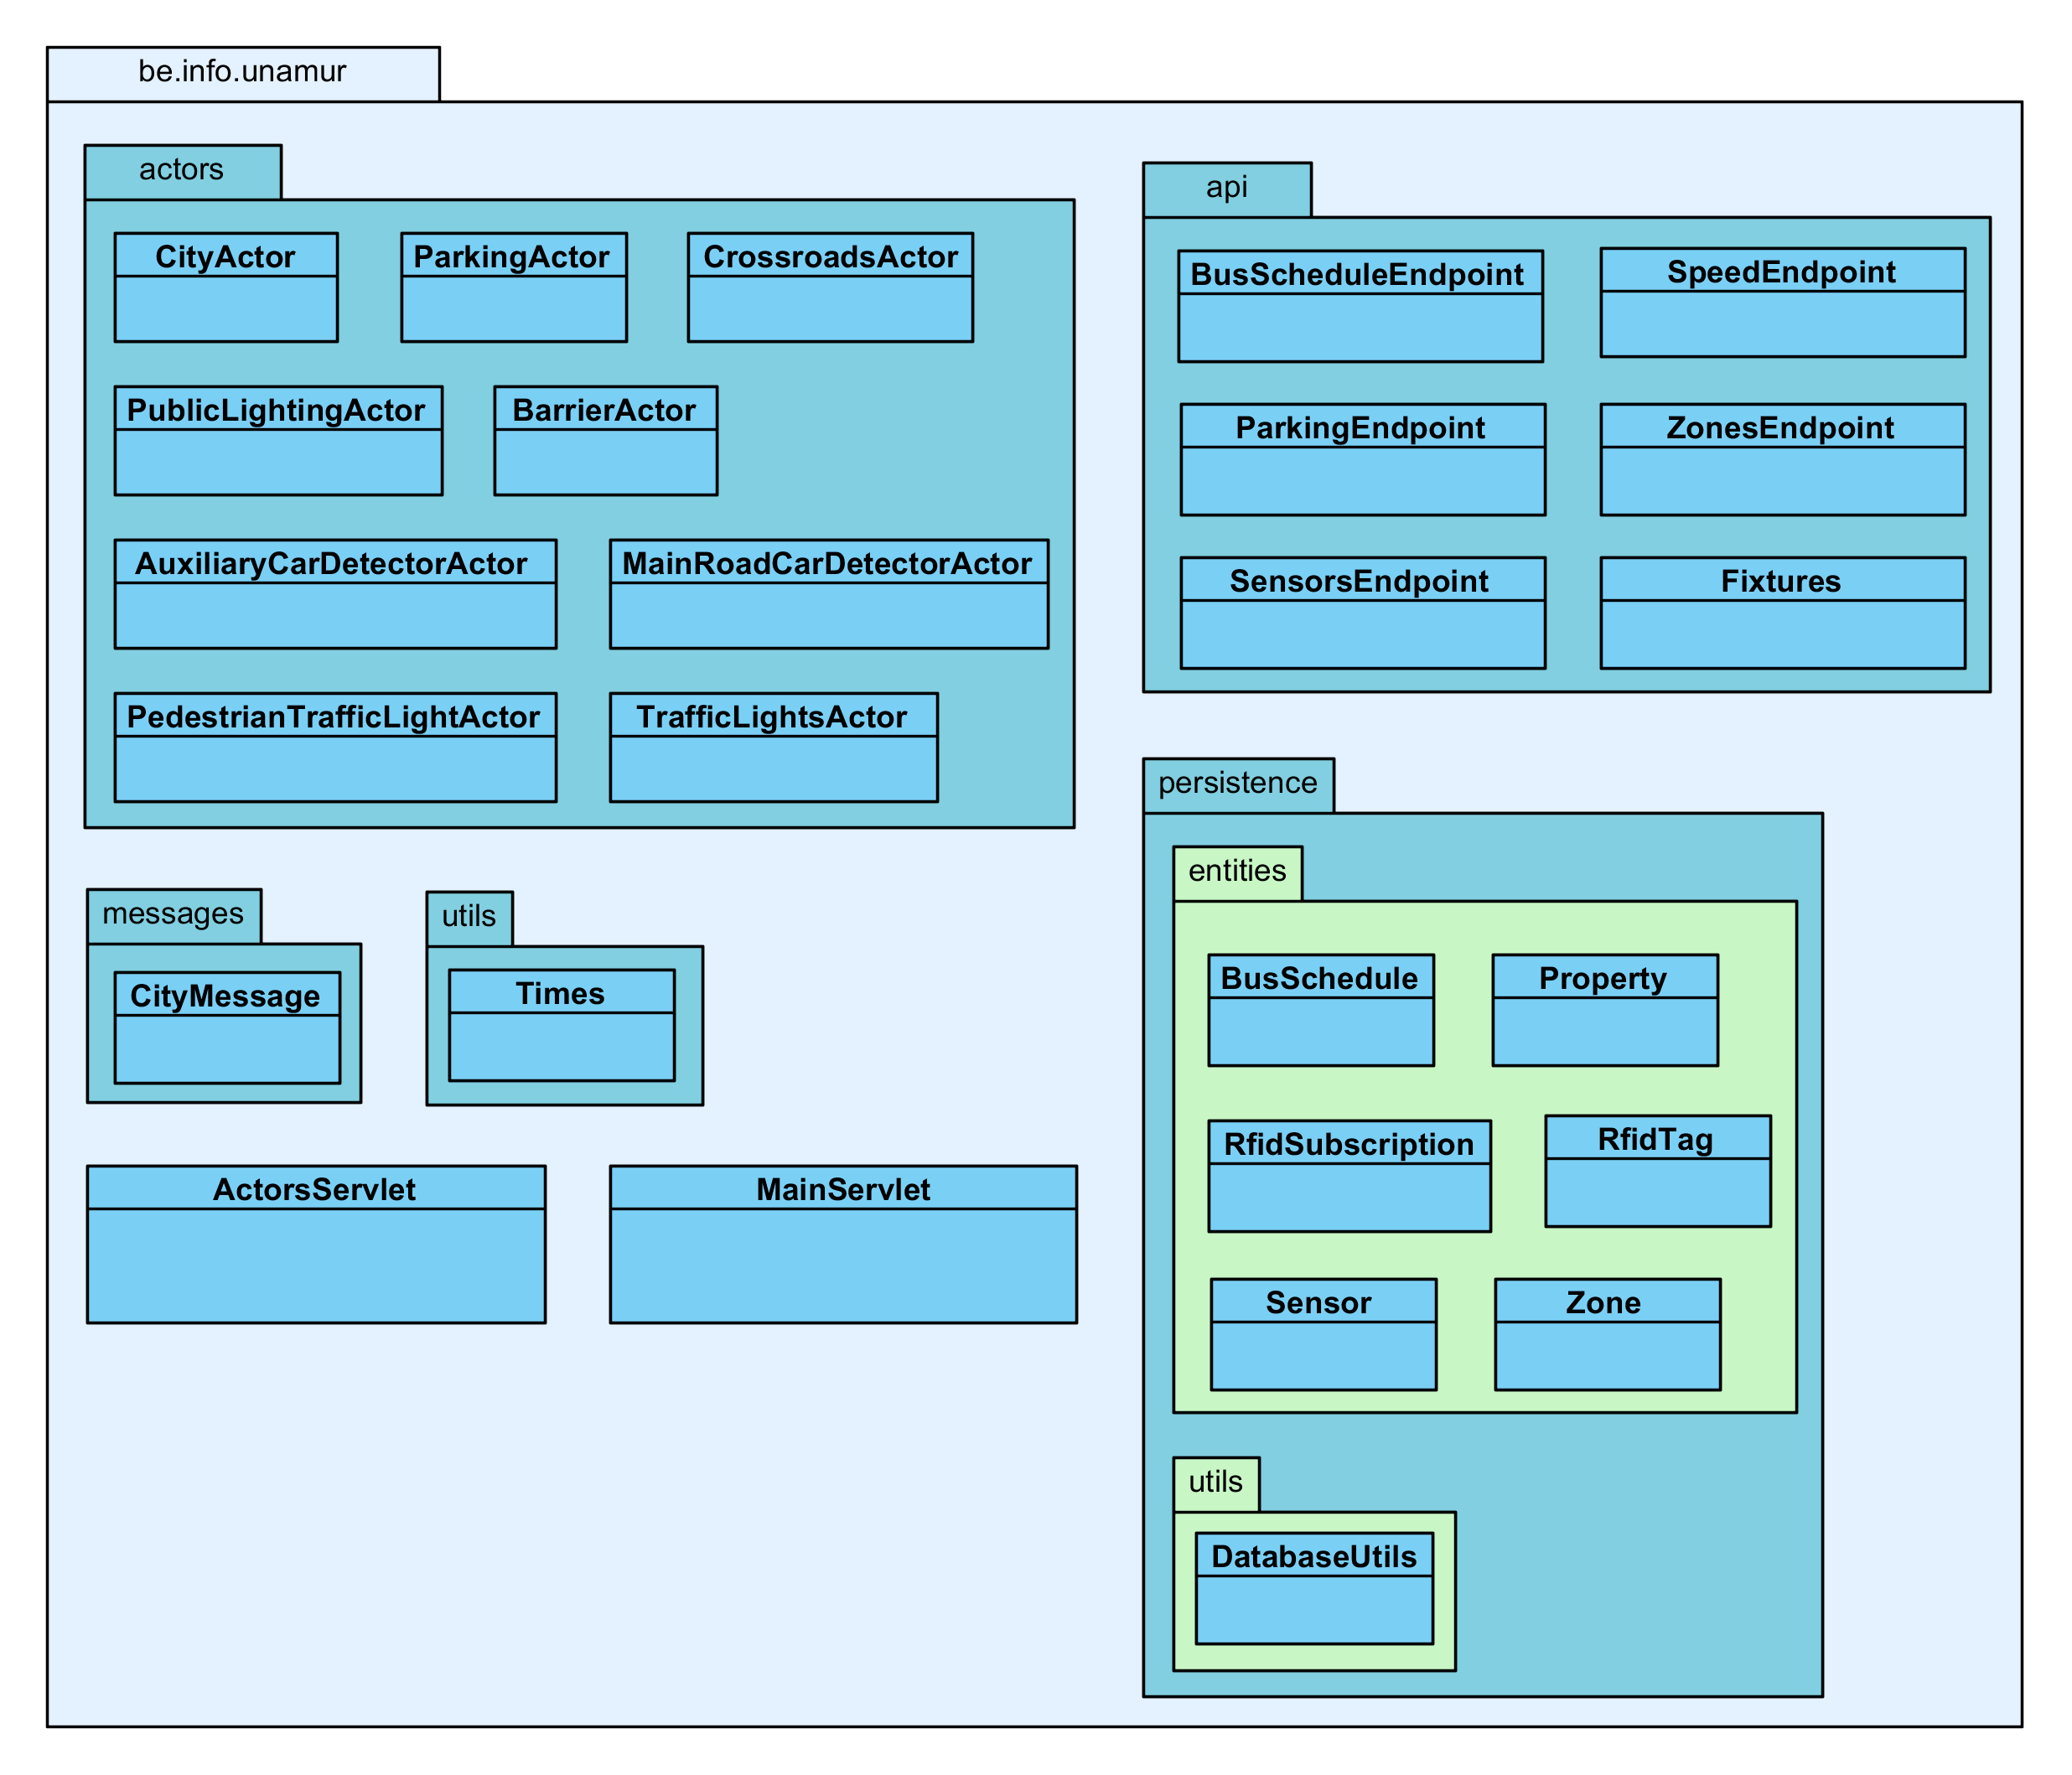
\includegraphics[width=\linewidth, height=\textheight,keepaspectratio]{img/diagramme-class-archi-logi}}

        \caption{Diagramme de class de l'architecture logicielle}
    \end{center}
\end{figure}

Intéressons-nous maintenant aux 3 composants principaux : le système d’acteurs, les services web et la « persistance » (c.-à-d. l’interaction avec la base de données).


\subsubsection{Système d'acteurs}\label{systeme-acteurs}
Pour contrôler le matériel (c.-à-d. les phidgets décrits ci-avant qui sont connectés au Raspberry Pi), nous basons la notion d’Acteurs proposée par la librairie Akka. Ainsi, chaque concept physique (la ville, le carrefour, les feux de signalisations, etc.) de notre maquette est représenté par un acteur. Cela nous a permis de faciliter grandement le code, de le rendre plus modulable et facile à faire évoluer.
Ce système d’Acteurs s’organise sous la forme d’un arbre qui peut être représenté de la façon suivante :
\begin{figure}[H]
    \begin{center}
        \frame{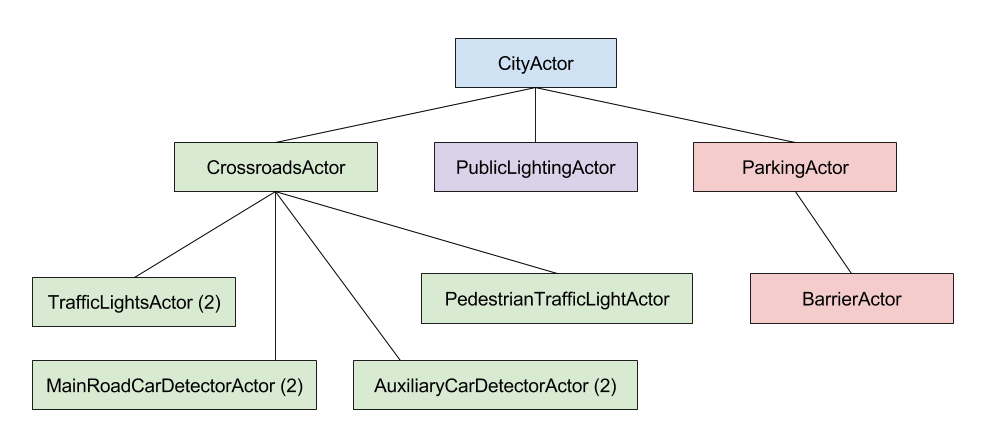
\includegraphics[width=\linewidth, height=\textheight,keepaspectratio]{img/systeme-acteurs-archi-logi}}

        \caption{Structure du système d'acteurs}
    \end{center}
\end{figure}
On remarque donc que la ville (\emph{CityActor}) est l’acteur principal ou aussi appelé le « maître », c’est lui qui est à la racine de notre système. Les sous-acteurs engendrés par celui-ci sont des composants plus petits à l’intérieur de la ville, c’est-à-dire le carrefour (\emph{CrossroadsActor}), le parking (\emph{ParkingActor}) et l’éclairage public (\emph{PublicLightingActor}).\\

Tout d’abord, il faut noter qu’il est possible de démarrer et d’arrêter tout le système d’acteurs. Ceci est réalisé en envoyant le message \emph{Initialize} à l’acteur principal qui va ensuite le propager dans tout l’arbre d’acteurs. De la même façon, s'ils ont été démarrés auparavant, il est possible de les stopper en envoyant le message \emph{Stop} à l’acteur principal qui le propagera de la même façon que pour le message de démarrage. Le fait d’initialiser des acteurs va ouvrir les connexions aux phidgets nécessaires, mais aussi ajouter les listeners et mettre en place une situation initiale (les feux de la voie principale au vert et ceux des auxiliaires au rouge, avec une inversion de situation toutes les 60 secondes et ce pendant 10 secondes avant que la situation ne revienne à la normale). Stopper les acteurs fera l’effet inverse.\\

Ensuite, l’acteur du carrefour pilote tous les composants nécessaires au bon fonctionnement du celui-ci :
\begin{itemize}
\item Les détecteurs de voitures sur la voie principale (\emph{MainRoadCarDetectorActor}). Comme expliqué dans la partie concernant le matériel, ces détecteurs sont au nombre de deux, un pour la voie principale côté Ouest et un pour la voie principale côté Est. Il y aura donc bien deux instanciations de l’acteur \emph{MainRoadCarDetectorActor}.
\item Les détecteurs de voitures sur la voie auxiliaire (\emph{AuxiliaryCarDetectorActor}). Similairement aux détecteurs de voitures, il existe deux capteurs, un pour le Nord et un pour le Sud, et donc deux instanciations de l’acteur \emph{AuxiliaryCarDetectorActor}.
\item Les feux de signalisations pour les voitures (un acteur \emph{TrafficLightsActor} par feu). Sur notre maquette, il existe 4 feux mais ceux des voies auxiliaires (Nord et Sud) et ceux des voies secondaires (Ouest et Est) fonctionnent respectivement en parallèle, uniquement deux instanciations de l’acteur \emph{TrafficLightsActor} sont dès lors nécessaires.
\item Les feux de signalisations pour les piétons (un acteur \emph{PedestrianTrafficLightActor} par feu). Uniquement les voies auxiliaires sont équipées de feux pour piétons fonctionnant en parallèle, il y aura donc une seule instanciation de l’acteur \emph{PedestrianTrafficLightActor}.
\end{itemize}

Le contrôle du carrefour part principalement de l’acteur qui gère celui-ci, en envoyant des messages aux sous-acteurs pour déléguer le travail (allumer et éteindre des feux, vérifier l’état des détecteurs de présences, etc.).\\

Le comportement général du carrefour est le suivant : lorsqu'un des capteurs sur l'une des voies auxiliaires détecte une voiture, les feux passent au vert sur les voies auxiliaires et au rouge sur la voie principal. Cependant, si une ou plusieurs voitures est(sont) détectée(s) sur la voie principale, un délais (de l'ordre de 4 secondes) est mis en place pour essayer de désengorger la voie principale dans un premier temps.
Les feux sur les voies auxiliaires restent au vert pendant 10 secondes puis passent au rouges et la voie principale est de nouveau ouverte. Si une voiture venait à nouveau à être détectée sur une des voies auxiliaires, elle devrait patienter un délais supplémentaire (de 20 secondes) avant de pouvoir passer.
Il va de soit que lorsque la voie principale est au vert et que les voies auxiliaires sont fermées, les passage piétons de ces dernières sont ouverts.\\

L’acteur pour le parking s’occupe principalement du lecteur RFID et aussi de contrôler la barrière en envoyant des messages à l’acteur correspondant à celle-ci (\emph{BarrierActor}). Ainsi, grâce à un listener sur le lecteur RFID, lorsqu’un tag est lu, si celui-ci est enregistré dans la base de données (voir ci 2.2.1.3), l’acteur envoie le message d’ouverture de la barrière du parking à l’acteur concerné. Quand le tag est perdu, il envoie le message de fermeture.\\

L’acteur pour l’éclairage public allume et éteint lorsqu’il est nécessaire les LEDs représentant ce même éclairage sur la maquette. Pour ce faire, un listener écoute les valeurs du capteur de luminosité et allume ou éteint certaines LEDs. Par exemple, si la valeur renvoyée par le capteur est élevée, les 3 LEDs seront allumées et inversement dans l’autre cas mais aussi avec des valeurs intermédiaires pour allumer 1 ou 2 LEDs.\\

Enfin, tous les messages échangés entre les acteurs sont définis dans la “case class” \emph{CityMessage}.


\subsubsection{Services web (API REST)}
L’API REST que nous avons mise en place est implémentée en se basant intégralement sur les outils proposés par Scalatra. Ainsi, il est facile de rajouter de nouveau point d’accès ou d’en supprimer. De plus la documentation de celle-ci est disponible sous format JSON et peut être visualisée en utilisant l’outil Swagger UI (c’est aussi pourquoi nous ne nous attarderons pas à documenter ici toute l’API).\\

Les points d’accès principaux sont les suivants :
\begin{center}
{\renewcommand{\arraystretch}{1.5}
\begin{longtable}{| p{.35\textwidth} | p{.59\textwidth} |}
    \hline
    \textbf{Nom} & \textbf{Description}\\
    \hline
    \emph{BusScheduleEndpoint} & Permet de récupérer et de modifier les informations des horaires de bus au sein de la ville.\\
    \hline
    \emph{ParkingEndpoint} & Permet de récupérer certaines informations concernant le parking (comme l’historique d’entrées/sorties ou le nombre de places disponibles).\\
    \hline
    \emph{SensorsEndpoint} & Donne accès aux informations concernant tous les capteurs implantés dans la ville : luminosité, présence, température, humidité, ...\\
    \hline
    \emph{SpeedEndpoint} & Sert principalement à récupérer la vitesse courante au sein de la ville.\\
    \hline
    \emph{ZonesEndpoint} & Permet de fermer et d’ouvrir certaines zones mais aussi de connaître lesquelles sont fermées. Un historique des fermetures et des ouvertures est également disponible.\\
    \hline
    \caption{Points d'accès de l'API REST}
\end{longtable}}
\end{center}
\vspace{-1cm}

\subsubsection{Persistence}
Pour communiquer avec notre base de données MySQL, nous nous somme appuyés sur la librairie ScalikeJDBC. Dans le package nommé \emph{entities}, se trouvent donc toutes les DAO nécessaires (chaque DAO correspondant à une table dans la base de données) :
\begin{center}
{\renewcommand{\arraystretch}{1.5}
\begin{longtable}{| p{.69\textwidth} | x{.25\textwidth} |}
    \hline
    \textbf{Nom} & \textbf{Schéma}\\
    \hline
    \emph{BusSchedule} (correspond à la table 'bus\_schedule') &
    \begin{minipage}{\linewidth}
        \centering
        \vspace{12pt}
        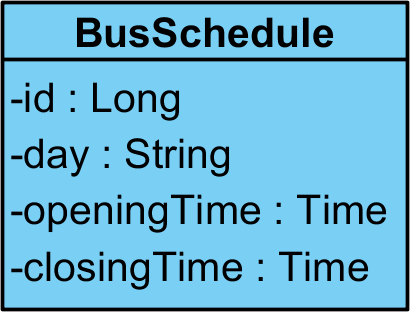
\includegraphics[scale=0.8]{img/bus-schedule}\par
        \vspace{12pt}
    \end{minipage}\\
    \hline
    \emph{Property} (correspond à la table 'properties') &
    \begin{minipage}{\linewidth}
        \centering
        \vspace{12pt}
        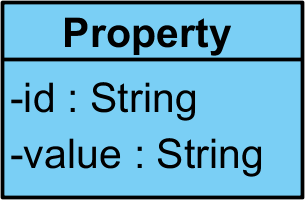
\includegraphics[scale=0.8]{img/property}\par
        \vspace{12pt}
    \end{minipage}\\
    \hline
    \emph{RfidSubscription} (correspond à la table 'rfid\_subscription') &
    \begin{minipage}{\linewidth}
        \centering
        \vspace{12pt}
        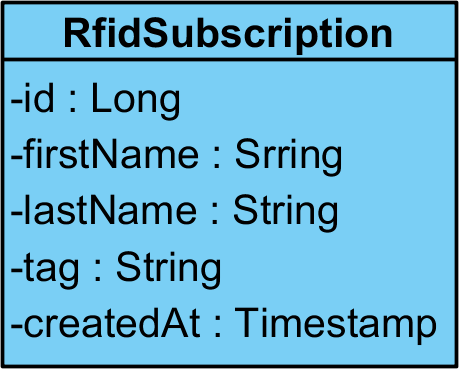
\includegraphics[scale=0.8]{img/rfid-sub}\par
        \vspace{12pt}
    \end{minipage}\\
    \hline
    \emph{RfidTag} (correspond à la table 'rfid\_tag') &
    \begin{minipage}{\linewidth}
        \centering
        \vspace{12pt}
        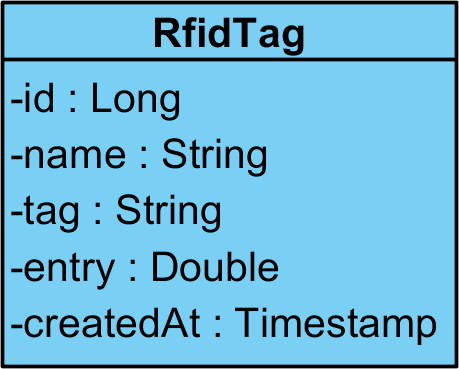
\includegraphics[scale=0.8]{img/rfid-tag}\par
        \vspace{12pt}
    \end{minipage}\\
    \hline
    \emph{Sensor} (correspond à la table 'sensors') &
    \begin{minipage}{\linewidth}
        \centering
        \vspace{12pt}
        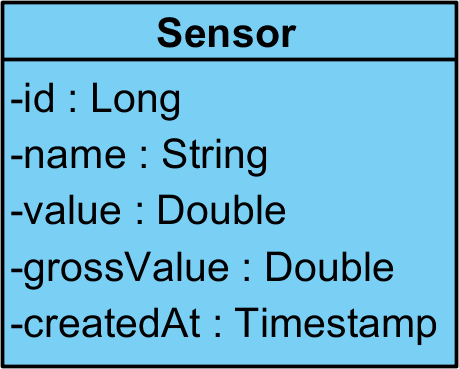
\includegraphics[scale=0.8]{img/sensor}\par
        \vspace{12pt}
    \end{minipage}\\
    \hline
    \emph{Zone} (correspond à la table 'zones') &
    \begin{minipage}{\linewidth}
        \centering
        \vspace{12pt}
        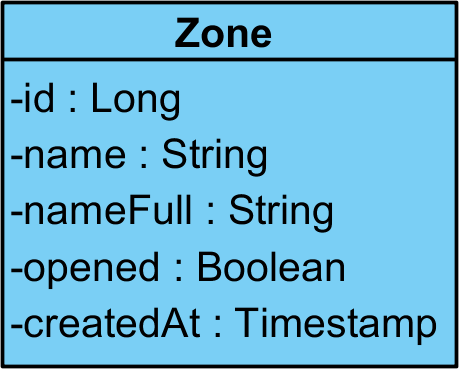
\includegraphics[scale=0.8]{img/zone}\par
        \vspace{12pt}
    \end{minipage}\\
    \hline
    \caption{Entités de la base de données}
\end{longtable}}
\end{center}
\vspace*{-0.7cm}
Les méthodes CRUD (et quelques autres qui nous sont utiles) se trouvent dans les objets "companions" correspondants à chaque DAO.